\chapter{Längenmessung}
\section{Motivation}
In einem Sägewerk ist die Messanlage ausgefallen. Euer Roboter muss jetzt das Messen übernehmen! Da es aufgrund der Maschinen im Sägewerk aus Sicherheitsgründen nicht möglich ist, sich frei zu bewegen, muss die Messung stationär erfolgen.

\begin{capfigure}[Messung Skizze]
	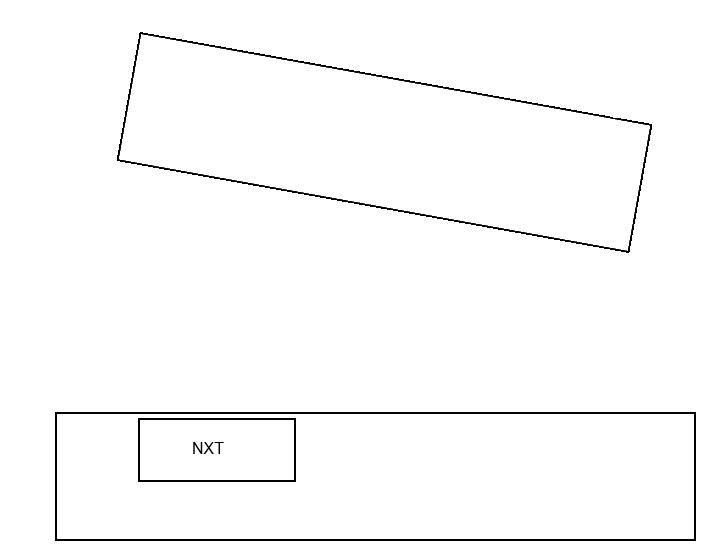
\includegraphics[width=10cm]{images/messen_skizze}
\end{capfigure}

\section{Aufgabenstellung}
Der Roboter soll die Länge des Holzstücks nur mit Hilfe des Ultraschallsensors messen. Während des Messens muss der Roboter fest an einer Stelle stehen. Der Roboter darf an eine beliebige Stelle innerhalb der Markierung gestellt werden. 

\subsection{Lösungshilfe}
Als Hilfe für die Lösung gibt es hier noch zwei Formeln.

\subsubsection{Variante A}
Wenn der Roboter bündig zu einem Ende des Objektes steht, kann man den Satz des Pythagoras verwenden.

$a^2 + b^2 + = c^2$

\begin{capfigure}[Pythagoras]
	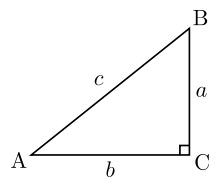
\includegraphics[width=6cm]{images/pythagoras.png}
\end{capfigure}

\clearpage
\subsubsection{Variante B}
Wenn der Roboter nicht bündig zum Anfang oder Ende des Objektes steht, dann kann der Kosinussatz verwendet werden.

$a^2 + b^2 - 2ab*cos\gamma = c^2$

\begin{capfigure}[Kosinussatz]
	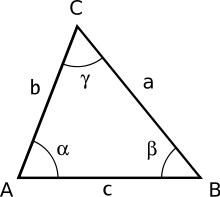
\includegraphics[width=6cm]{images/kosinus.png}
\end{capfigure}

Zusatzaufgabe: Berechnet die Fläche des Objekts. Hierfür muss das Objekt mit der Spitze zum Roboter liegen. 

Anmerkung: Um die Variante B mit NXT-G zu lösen muss auf ein Plugin zurückgegriffen werden, dass die Kosinus-Funktion bereitstellt. 

\section{Lösung}
\subsection{Länge messen}
Bei der Lösung für die Berechnung verwenden wir den Kosinussatz. Hierfür verwenden wir ein Plugin für NXT-G. Wir messen die Distanz zu den beiden Enden des Objekts und den Winkel dazwischen. Danach wird lediglich der Kosinussatz angewendet. $c = \sqrt{a^2 + b^2 - 2ab*cos\gamma}$ liefert uns die Länge des Objektes.

\subsection{Fläche messen}
Das Messend er Fläche läuft analog zu dem Messen der Länge. Es wird gemessen bis zur Ecke des Objekts(wenn die Distanz wieder größer wird). Es wird zweimal die Länge berechnet und daraus dann die Fläche.

Beide Lösungen sind auf der DVD unter \textit{Lösungen/Messen} zu finden.